% Poster: Binary Person Segmentation on Penn-Fudan (IIT Patna, iMPACT format)
% Build:  pdflatex poster.tex  &&  pdftoppm -png -r 110 poster.pdf poster
\documentclass{article}
\usepackage[paperwidth=118.9cm,paperheight=66.9cm,margin=1.1cm]{geometry}
\usepackage[T1]{fontenc}
\usepackage{mathptmx}
\usepackage[most]{tcolorbox}
\usepackage{graphicx}
\usepackage{xcolor}
\usepackage{tabularx}
\usepackage{booktabs}
\usepackage{amsmath}
\usepackage{enumitem}
\pagestyle{empty}
\setlength{\parindent}{0pt}

\definecolor{navy}{HTML}{1F3A5F}
\definecolor{cream}{HTML}{FBE9DC}
\definecolor{panelblue}{HTML}{EAF3FB}
\definecolor{panelpeach}{HTML}{FDEFE3}
\definecolor{panelgreen}{HTML}{EAF7EE}
\definecolor{algoink}{HTML}{20304A}

\newtcolorbox{panel}[2][panelblue]{enhanced, colback=#1, colframe=navy, boxrule=2.2pt, arc=10pt, left=12pt, right=12pt, top=10pt, bottom=10pt, width=#2}
\newcommand{\panelhead}[1]{{\color{navy}\bfseries\fontsize{30}{34}\selectfont #1\par\vspace{6pt}}}
\newcommand{\bodytext}{\fontsize{20}{26}\selectfont}
\newcommand{\smalltext}{\fontsize{17.5}{23}\selectfont}
\setlist{nosep, leftmargin=1.6em}

\begin{document}
{\color{algoink}%
% ============================ HEADER ============================
\begin{tcolorbox}[enhanced, colback=cream, colframe=navy, boxrule=2.5pt, arc=8pt, left=10pt, right=10pt, top=8pt, bottom=8pt]
\begin{minipage}{0.105\textwidth}\centering
\includegraphics[height=4.4cm]{logo_iitpatna.png}\end{minipage}%
\begin{minipage}{0.79\textwidth}\centering
{\color{navy}\bfseries\fontsize{33}{39}\selectfont Binary Person Segmentation on Penn-Fudan with U-Net, Augmentation and Synthetic\\[2pt] Reflection/Shadow Distractors\par}
\vspace{7pt}
{\color{algoink}\fontsize{22}{27}\selectfont Rahul Kumar Sahoo, \hspace{2pt}Roll No.\ 2401CS09\\[2pt]
Department of Computer Science and Engineering, Indian Institute of Technology Patna\par}
\end{minipage}%
\begin{minipage}{0.105\textwidth}\centering
\includegraphics[height=3.2cm]{logo_impact.png}\end{minipage}
\end{tcolorbox}

\vspace{8pt}
% ============================ COLUMNS ============================
\begin{minipage}[t]{0.325\textwidth}
\vspace{0pt}
\begin{panel}[panelblue]{\linewidth}
\bodytext
\panelhead{Abstract}
We segment pedestrians in the 170-image Penn-Fudan dataset, merging all people into one binary mask. With one frozen 102/34/34 split, validation-only model selection and a single test evaluation, we compare baselines, U-Net variants, a ResNet34-encoder U-Net and DeepLabV3 over three seeds. The pretrained encoder gives the largest gain (+0.0736 mean per-image IoU); fine-tuned DeepLabV3 scores best (0.7973). Training with synthetic reflection and shadow distractors cuts the ResNet34 false-positive rate on them from 0.1314 to 0.0273.

\vspace{9pt}
\panelhead{Introduction}
\begin{itemize}\setlength\itemsep{5pt}
\item Person segmentation labels every pixel as person or background. It supports pedestrian analysis, editing and privacy blurring.
\item Small datasets make gains hard to trust: one lucky seed can look like progress.
\item Segmenters may also call mirror images or person-shaped shadows people, but Penn-Fudan has no such cases to test this.
\end{itemize}

\vspace{9pt}
\panelhead{Problem Statement}
Given an RGB street photo, predict a binary mask of all pedestrians, training on 102 images, so that test IoU clearly beats trivial baselines; and measure how often synthetic reflection- and shadow-like regions pasted on the background are wrongly called person.
\end{panel}
\end{minipage}%
\begin{minipage}[t]{0.375\textwidth}
\vspace{0pt}\hspace{6pt}\begin{panel}[panelpeach]{\dimexpr\linewidth-6pt}
\bodytext
\panelhead{Key Contributions}
\begin{itemize}\setlength\itemsep{4pt}
\item 27 runs (9 configs $\times$ 3 seeds) and 3 baselines under one frozen, leak-free protocol.
\item Seed spread and paired bootstrap CIs; mild augmentation: +0.0271 [0.0086, 0.0446].
\item Six synthetic distractors on background only, scored by a false-positive rate FP$_D$.
\item Error analysis: several of the worst false positives are unlabelled people.
\end{itemize}

\vspace{7pt}
\panelhead{Methodology}
U-Net (7.76\,M), ResNet34-encoder U-Net (24.52\,M) and DeepLabV3-ResNet50 (42.00\,M), trained with AdamW on BCE or BCE\,+\,Dice; only training images are augmented.

\vspace{5pt}
{\smalltext {\color{navy}\bfseries Training phase (blue): all fitting uses the 102 training images}\\
{\color{navy}\bfseries Evaluation phase (peach): no fitting, test set used once}\par}
\vspace{6pt}
\begin{center}
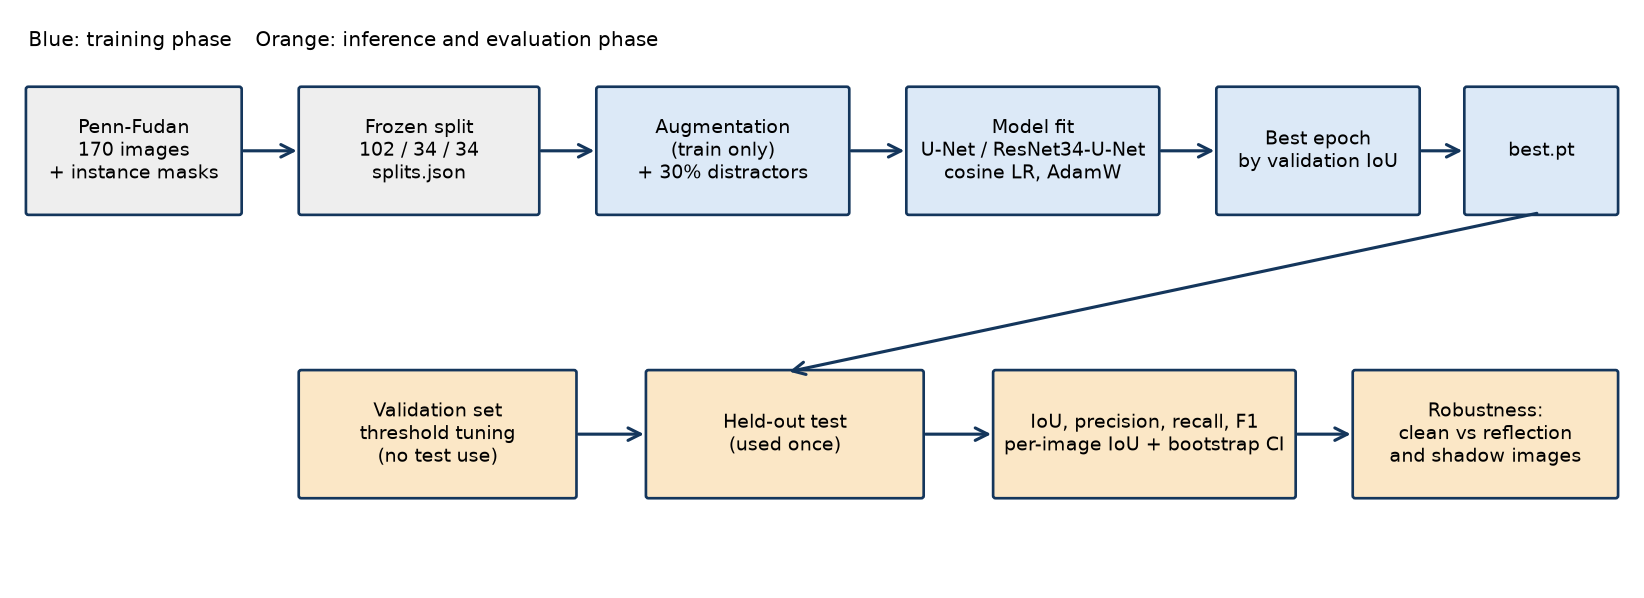
\includegraphics[width=0.90\linewidth]{architecture.png}\\[5pt]
{\smalltext \textbf{Figure 1:} End-to-end architecture of the study pipeline\par}
\end{center}
\vspace{7pt}
\begin{tcolorbox}[enhanced, colback=white, colframe=navy, boxrule=1.6pt, arc=6pt, left=10pt, right=10pt, top=8pt, bottom=8pt]
{\fontsize{16.5}{22}\selectfont\ttfamily\color{algoink}
\textbf{Algorithm 1: Leak-free multi-seed study}\\[3pt]
\textbf{Input:} images D; frozen split D\textsubscript{tr}/D\textsubscript{val}/D\textsubscript{te}; configs C; seeds S = \{20261103, 1, 2\}\\
1. Binarise masks (mask > 0); resize to 256$\times$256.\\
2. \textbf{for} c in C, s in S: train 100 epochs on augmented D\textsubscript{tr} (+ distractors, p = 0.3); keep best D\textsubscript{val}-IoU epoch.\\
3. Choose t* on D\textsubscript{val} only; test once on D\textsubscript{te}: IoU, P, R, F1, bootstrap CI.\\
4. Paste 6 distractor types on D\textsubscript{te} backgrounds; report FP$_D$.\\
5. Report mean $\pm$ std over seeds; paired bootstrap differences.\par}
\end{tcolorbox}
\end{panel}
\end{minipage}%
\begin{minipage}[t]{0.30\textwidth}
\vspace{0pt}\hspace{6pt}\begin{panel}[panelgreen]{\dimexpr\linewidth-6pt}
\bodytext
\panelhead{Result and Discussion}
{\smalltext \textbf{Table 1:} Test results at t = 0.5 (mean $\pm$ std, 3 seeds)\par}
\vspace{5pt}
\begin{center}
\resizebox{0.98\linewidth}{!}{%
\begin{tabular}{@{}lccc@{}}
\toprule
\textbf{Model} & \textbf{Mean image IoU} & \textbf{Pooled IoU} & \textbf{FP$_D$} \\
\midrule
pixel RF & 0.2713 & 0.2645 & -- \\
U-Net baseline & 0.6893 $\pm$ 0.0146 & 0.6564 & 0.1465 \\
U-Net + mild aug. & 0.7164 $\pm$ 0.0015 & 0.6831 & 0.1470 \\
ResNet34-U-Net & 0.7895 $\pm$ 0.0094 & 0.7695 & 0.1314 \\
ResNet34 + distr. & 0.7903 $\pm$ 0.0052 & 0.7668 & 0.0273 \\
DeepLab zero-shot & 0.7567 & 0.7343 & 0.1666 \\
DeepLab fine-tuned & \textbf{0.7973 $\pm$ 0.0017} & 0.7801 & 0.1306 \\
\bottomrule
\end{tabular}}
\end{center}
\vspace{8pt}
\begin{center}
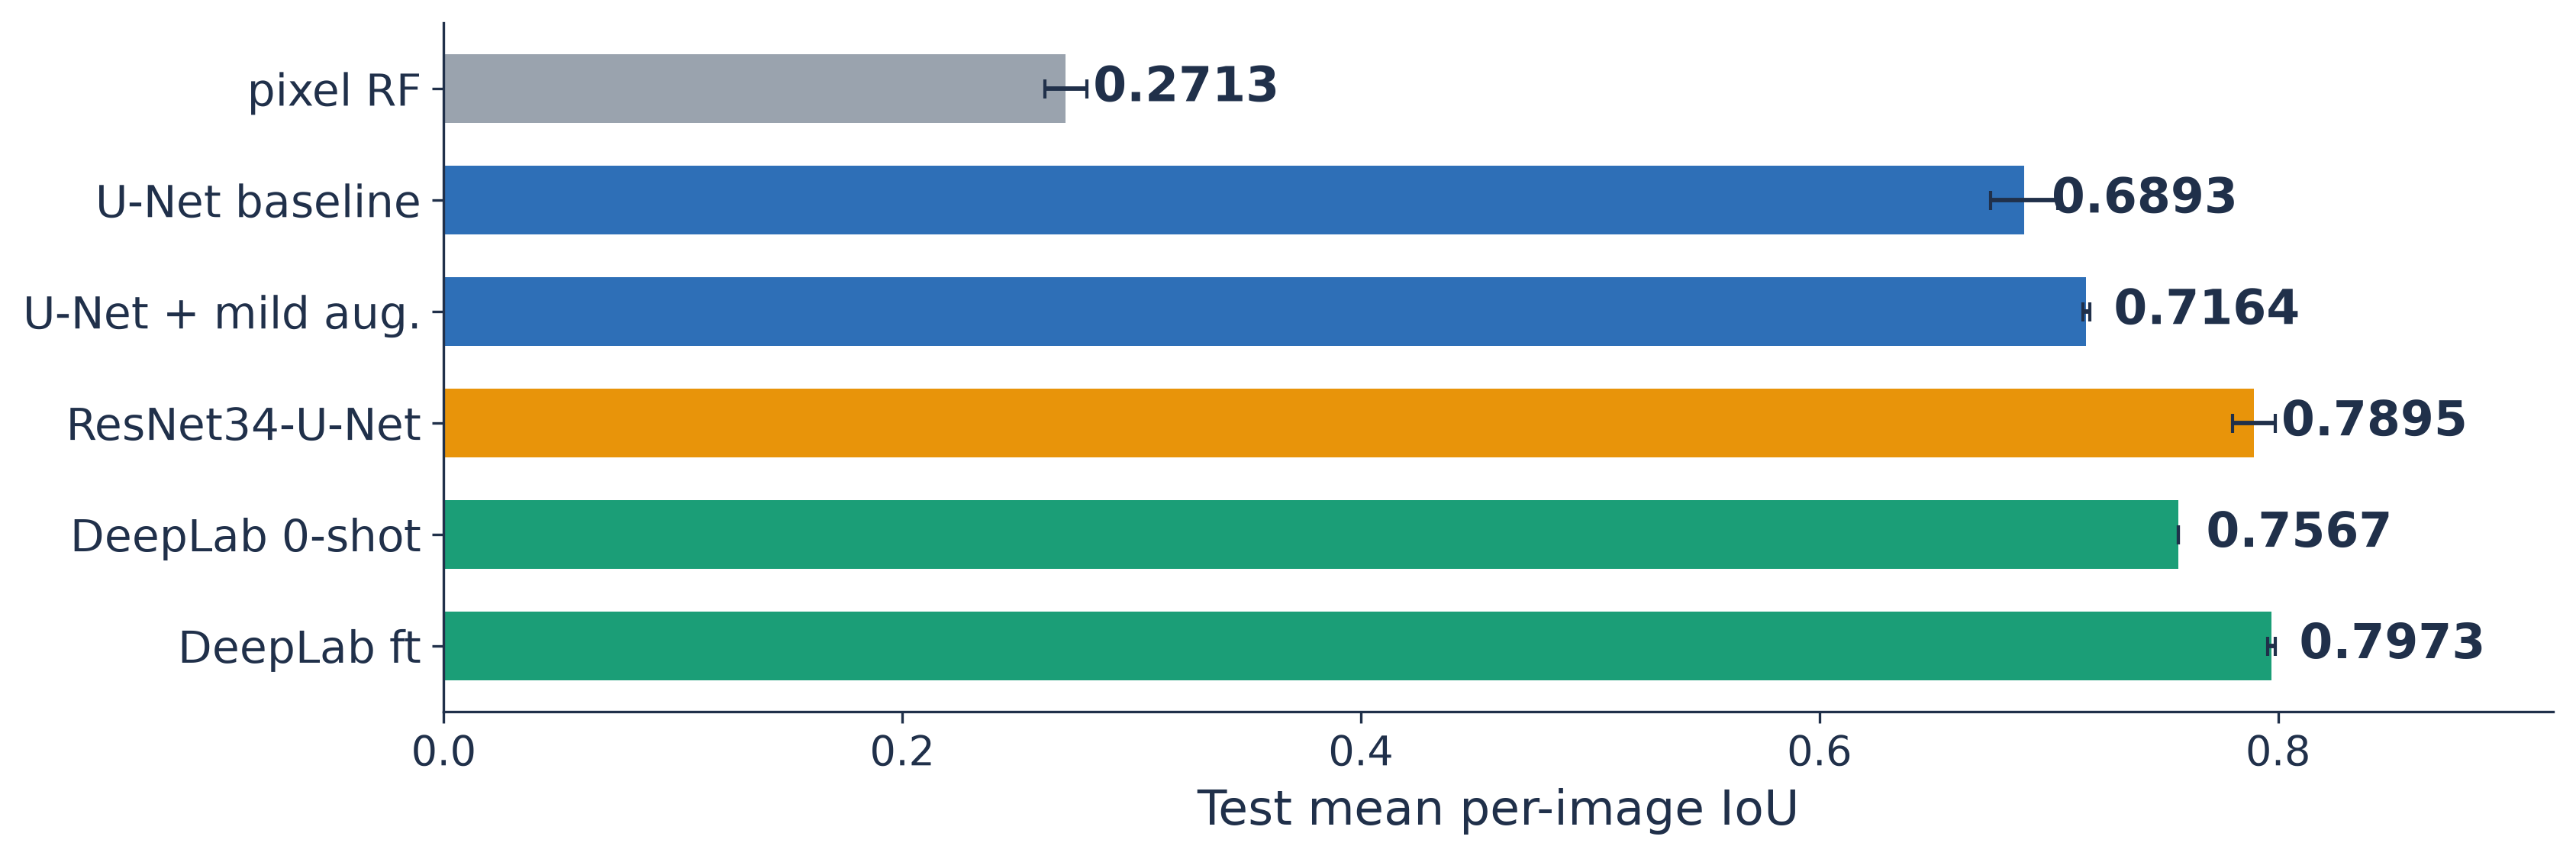
\includegraphics[width=0.99\linewidth]{poster_iou.png}\\[3pt]
{\smalltext (a) Test mean per-image IoU\par}
\vspace{6pt}
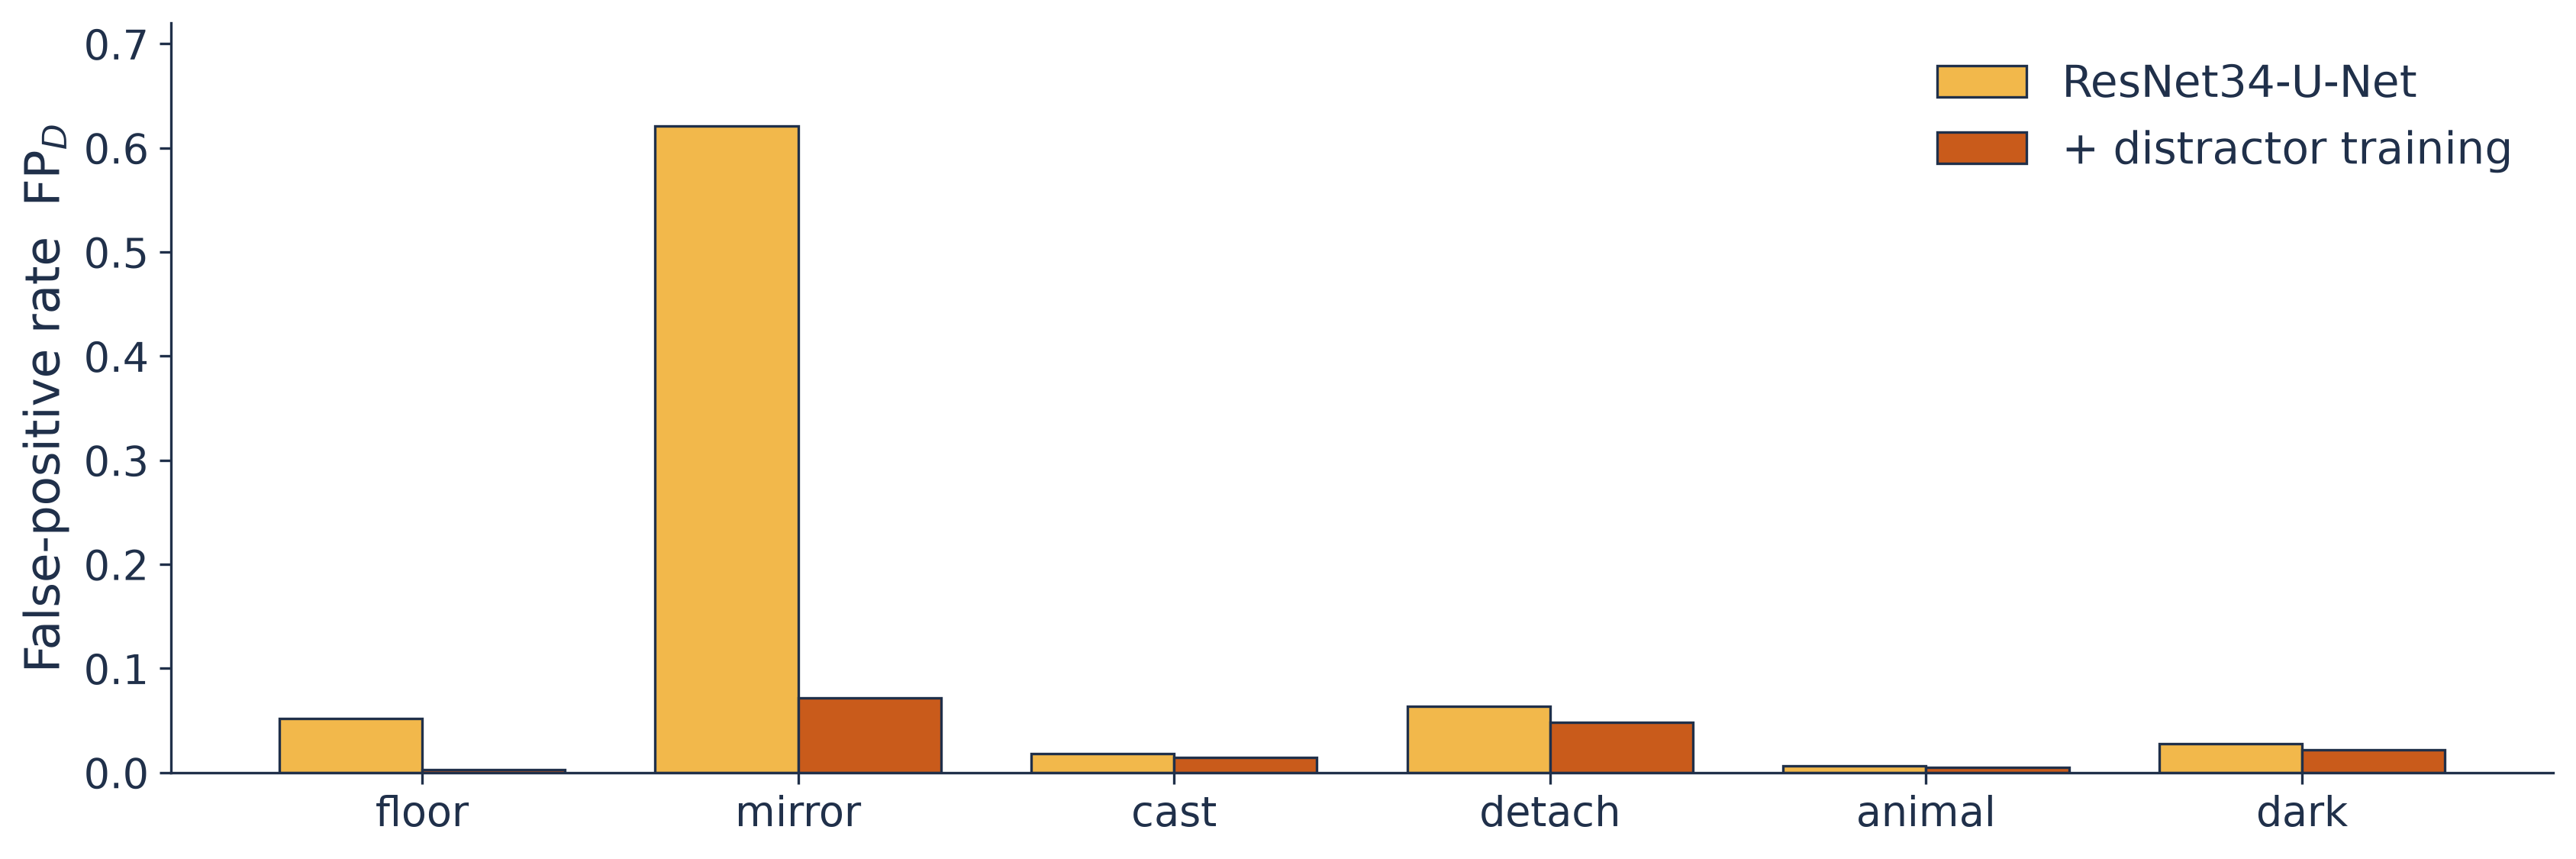
\includegraphics[width=0.99\linewidth]{poster_fpd.png}\\[3pt]
{\smalltext (b) Distractor false-positive rate FP$_D$\par}
\vspace{4pt}
{\smalltext \textbf{Figure 2:} Test IoU by model and distractor robustness\par}
\end{center}
\vspace{6pt}
\panelhead{Conclusion}
Pretrained encoders matter most; distractor training helps ResNet34 (FP$_D$ 0.1314 $\to$ 0.0273) at almost no clean cost. Real reflections remain untested.
\end{panel}
\end{minipage}

\vspace{8pt}
% ============================ FOOTER ============================
\begin{tcolorbox}[enhanced, colback=cream, colframe=navy, boxrule=2.5pt, arc=8pt, left=12pt, right=12pt, top=8pt, bottom=8pt]
\begin{minipage}{0.075\textwidth}{\color{navy}\bfseries\fontsize{24}{28}\selectfont References\par}\end{minipage}%
\begin{minipage}{0.615\textwidth}{\fontsize{15.5}{20.5}\selectfont
[1] L. Wang, J. Shi, G. Song, I.-F. Shen, ``Object detection combining recognition and segmentation,'' ACCV, 2007. \quad
[2] O. Ronneberger, P. Fischer, T. Brox, ``U-Net: Convolutional networks for biomedical image segmentation,'' MICCAI, 2015.\\[3pt]
[3] K. He, X. Zhang, S. Ren, J. Sun, ``Deep residual learning for image recognition,'' CVPR, 2016. \quad
[4] L.-C. Chen et al., ``Rethinking atrous convolution for semantic image segmentation,'' arXiv:1706.05587, 2017.\par}\end{minipage}%
\begin{minipage}{0.21\textwidth}\centering{\fontsize{16.5}{21}\selectfont \textbf{Code and data instructions:}\\{\color{navy}\bfseries github.com/Rahul-1-eng/\\person-segmentation-pennfudan\par}}\end{minipage}%
\begin{minipage}{0.07\textwidth}\centering
\includegraphics[height=3.4cm]{qr_github.png}\end{minipage}
\end{tcolorbox}
}
\end{document}
